\chapter{Derivadas parciais}

Sejam \(f:D_f\subset\R^2 \to \R\) e \((x_0,y_0)\in D_f\). Fixado \(y=y_0\), podemos considerar a função de uma variável \(g(x) = f(x,y_0)\). Assim
\begin{definition}
    Se \(g'(x_0)\) existe, então \[\frac{\partial f}{\partial x} f(x_0,y_0) = g'(x_0)\] é a derivada parcial de \(f\) em relação a \(x\) no ponto \((x_0,y_0)\). \index{Derivada parcial}
\end{definition}

Note que \[\frac{\partial f}{\partial x} (x_0,y_0) = g'(x_0) = \lim_{x\to x_0} \frac{g(x) - g(x_0)}{x-x_0} = \lim_{x\to x_0} \frac{f(x,y_0) - f(x_0,y_0)}{x-x_0} = \lim_{h\to 0} \frac{f(x_0 + h,y_0) - f(x_0,y_0)}{h}.\]

Note que o gráfico da função \(g(x) = f(x,y_0)\) é a interseção do plano \(y = y_0\) com o gráfico de \(f\).
    \begin{figure}[htbp]
        \centering
        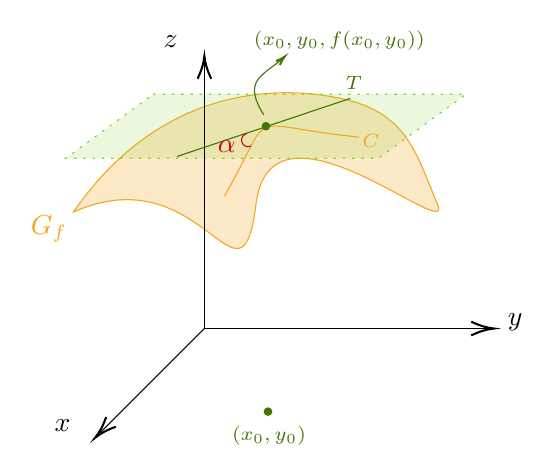
\begin{tikzpicture}[x=0.75pt,y=0.75pt,yscale=-1,xscale=1]
           %Curve Lines [id:da6266193197651527] 
            \draw [color={rgb, 255:red, 245; green, 166; blue, 35 }  ,draw opacity=1 ][fill={rgb, 255:red, 245; green, 166; blue, 35 }  ,fill opacity=0.25 ]   (136.27,144.27) .. controls (179.6,81.6) and (238.27,82.93) .. (268.27,90.27) .. controls (298.27,97.6) and (302.27,118.93) .. (311.6,140.27) .. controls (320.93,161.6) and (231.6,81.6) .. (224.27,140.27) .. controls (216.93,198.93) and (198.93,116.27) .. (136.27,144.27) -- cycle ;
            %Shape: Rectangle [id:dp819297825887712] 
            \draw  [color={rgb, 255:red, 126; green, 211; blue, 33 }  ,draw opacity=1 ][fill={rgb, 255:red, 126; green, 211; blue, 33 }  ,fill opacity=0.15 ][dash pattern={on 0.84pt off 2.51pt}] (174.8,87.5) -- (325.42,87.5) -- (283.25,118.32) -- (132.63,118.32) -- cycle ;
            %Straight Lines [id:da7425257041932752] 
            \draw    (199.37,200.38) -- (199.37,71.11) ;
            \draw [shift={(199.37,69.11)}, rotate = 90] [color={rgb, 255:red, 0; green, 0; blue, 0 }  ][line width=0.75]    (10.93,-3.29) .. controls (6.95,-1.4) and (3.31,-0.3) .. (0,0) .. controls (3.31,0.3) and (6.95,1.4) .. (10.93,3.29)   ;
            %Straight Lines [id:da4106868248301041] 
            \draw    (199.37,200.38) -- (336.89,200.38) ;
            \draw [shift={(338.89,200.38)}, rotate = 180] [color={rgb, 255:red, 0; green, 0; blue, 0 }  ][line width=0.75]    (10.93,-3.29) .. controls (6.95,-1.4) and (3.31,-0.3) .. (0,0) .. controls (3.31,0.3) and (6.95,1.4) .. (10.93,3.29)   ;
            %Straight Lines [id:da7309914377202636] 
            \draw    (199.37,200.38) -- (148.05,251.7) ;
            \draw [shift={(146.64,253.11)}, rotate = 315] [color={rgb, 255:red, 0; green, 0; blue, 0 }  ][line width=0.75]    (10.93,-3.29) .. controls (6.95,-1.4) and (3.31,-0.3) .. (0,0) .. controls (3.31,0.3) and (6.95,1.4) .. (10.93,3.29)   ;
            %Curve Lines [id:da17297484071125124] 
            \draw [color={rgb, 255:red, 245; green, 166; blue, 35 }  ,draw opacity=1 ]   (209,136.68) .. controls (234.5,92.32) and (215.5,102.18) .. (274,108.18) ;
            %Shape: Circle [id:dp1482658967021505] 
            \draw  [draw opacity=0][fill={rgb, 255:red, 65; green, 117; blue, 5 }  ,fill opacity=1 ] (226.93,102.91) .. controls (226.93,101.76) and (227.87,100.82) .. (229.02,100.82) .. controls (230.18,100.82) and (231.11,101.76) .. (231.11,102.91) .. controls (231.11,104.06) and (230.18,105) .. (229.02,105) .. controls (227.87,105) and (226.93,104.06) .. (226.93,102.91) -- cycle ;
            %Shape: Circle [id:dp7645444717153175] 
            \draw  [draw opacity=0][fill={rgb, 255:red, 65; green, 117; blue, 5 }  ,fill opacity=1 ] (227.93,240.41) .. controls (227.93,239.26) and (228.87,238.32) .. (230.02,238.32) .. controls (231.18,238.32) and (232.11,239.26) .. (232.11,240.41) .. controls (232.11,241.56) and (231.18,242.5) .. (230.02,242.5) .. controls (228.87,242.5) and (227.93,241.56) .. (227.93,240.41) -- cycle ;
            %Curve Lines [id:da25128294727881173] 
            \draw [color={rgb, 255:red, 65; green, 117; blue, 5 }  ,draw opacity=1 ]   (228,97.45) .. controls (217.55,80.82) and (227.41,78.64) .. (236.56,70.75) ;
            \draw [shift={(238,69.45)}, rotate = 136.55] [color={rgb, 255:red, 65; green, 117; blue, 5 }  ,draw opacity=1 ][line width=0.75]    (4.37,-1.32) .. controls (2.78,-0.56) and (1.32,-0.12) .. (0,0) .. controls (1.32,0.12) and (2.78,0.56) .. (4.37,1.32)   ;
            %Straight Lines [id:da37877094571494097] 
            \draw [color={rgb, 255:red, 65; green, 117; blue, 5 }  ,draw opacity=1 ]   (186.25,117.48) -- (269.75,89.48) ;
            %Shape: Arc [id:dp3727122850882745] 
            \draw  [draw opacity=0] (221.87,112.44) .. controls (220.4,113.18) and (218.6,112.67) .. (217.74,111.25) .. controls (216.83,109.75) and (217.31,107.8) .. (218.81,106.89) .. controls (219.13,106.69) and (219.48,106.56) .. (219.83,106.49) -- (220.45,109.61) -- cycle ; \draw  [color={rgb, 255:red, 208; green, 2; blue, 27 }  ,draw opacity=1 ] (221.87,112.44) .. controls (220.4,113.18) and (218.6,112.67) .. (217.74,111.25) .. controls (216.83,109.75) and (217.31,107.8) .. (218.81,106.89) .. controls (219.13,106.69) and (219.48,106.56) .. (219.83,106.49) ;  

            % Text Node
            \draw (125.98,243) node [anchor=north west][inner sep=0.75pt]  [font=\normalsize]  {$x$};
            % Text Node
            \draw (178.48,58.05) node [anchor=north west][inner sep=0.75pt]  [font=\normalsize]  {$z$};
            % Text Node
            \draw (344.37,191.84) node [anchor=north west][inner sep=0.75pt]  [font=\normalsize]  {$y$};
            % Text Node
            \draw (114.5,144.6) node [anchor=north west][inner sep=0.75pt]    {$\textcolor[rgb]{0.96,0.65,0.14}{G}\textcolor[rgb]{0.96,0.65,0.14}{_{f}}$};
            % Text Node
            \draw (266.25,77.6) node [anchor=north west][inner sep=0.75pt]  [font=\scriptsize,color={rgb, 255:red, 65; green, 117; blue, 5 }  ,opacity=1 ]  {$T$};
            % Text Node
            \draw (274.2,105.33) node [anchor=north west][inner sep=0.75pt]  [font=\scriptsize]  {$\textcolor[rgb]{0.96,0.65,0.14}{C}$};
            % Text Node
            \draw (211.5,246.2) node [anchor=north west][inner sep=0.75pt]  [font=\scriptsize]  {$\textcolor[rgb]{0.25,0.46,0.02}{(}\textcolor[rgb]{0.25,0.46,0.02}{x}\textcolor[rgb]{0.25,0.46,0.02}{_{0}}\textcolor[rgb]{0.25,0.46,0.02}{,y}\textcolor[rgb]{0.25,0.46,0.02}{_{0}}\textcolor[rgb]{0.25,0.46,0.02}{)}$};
            % Text Node
            \draw (222,55.7) node [anchor=north west][inner sep=0.75pt]  [font=\scriptsize]  {$\textcolor[rgb]{0.25,0.46,0.02}{(}\textcolor[rgb]{0.25,0.46,0.02}{x}\textcolor[rgb]{0.25,0.46,0.02}{_{0}}\textcolor[rgb]{0.25,0.46,0.02}{,y}\textcolor[rgb]{0.25,0.46,0.02}{_{0}}\textcolor[rgb]{0.25,0.46,0.02}{,f}\textcolor[rgb]{0.25,0.46,0.02}{(}\textcolor[rgb]{0.25,0.46,0.02}{x}\textcolor[rgb]{0.25,0.46,0.02}{_{0}}\textcolor[rgb]{0.25,0.46,0.02}{,y}\textcolor[rgb]{0.25,0.46,0.02}{_{0}}\textcolor[rgb]{0.25,0.46,0.02}{)}\textcolor[rgb]{0.25,0.46,0.02}{)}$};
            % Text Node
            \draw (204.59,108.43) node [anchor=north west][inner sep=0.75pt]    {$\textcolor[rgb]{0.82,0.01,0.11}{\alpha }$};
        \end{tikzpicture}
        \caption{Interpretação geométrica da derivada}
        \label{fig:derivada}
    \end{figure}

    Dessa forma, \(\frac{\partial f}{\partial x}(x_0,y_0) = g'(x_0)\) é o coeficiente angular da reta tangente \(T\) à curva \(C\) no ponto \((x_0,y_0,f(x_0,y_0))\). Ou seja, \[\frac{\partial f}{\partial x}(x_0,y_0) = \tan(\alpha).\]

    Seja \(A\subset D_f\) o conjunto dos pontos \((x,y)\) tais que \(\frac{\partial f}{\partial x}(x,y)\) existe. Assim, fica bem definida uma função \(\frac{\partial f}{\partial x} : A \subset \R^2 \to \R\) dada por \[\frac{\partial f}{\partial x}(x,y) = \lim_{h\to 0} \frac{f(x+h,y) - f(x,y)}{h}.\] Chamamos tal função de \textbf{derivada parcial} (de 1ª ordem) de \(f\) em relação a \(x\). 
    
    De forma análoga definimos a derivada parcial de \(f\) em relação a \(y\) no ponto \(x_0,y\):
        \begin{itemize}
            \item Fixamos \(x = x_0\);
            \item tomamos \(h(y) = f(x_0,y)\);
            \item definimos \[\frac{\partial f}{\partial y}(x_0,y_0) = h'(y_0) = \lim_{y\to y_0} \frac{h(y) - h(y_0)}{y-y_0} = \lim_{y\to y_0} \frac{f(x_0,y) - f(x_0,y_0)}{y-y_0} = \lim_{h\to 0} \frac{f(x_0,y_0 + h) - f(x_0,y_0)}{h}. \]
        \end{itemize}

\begin{exercise}
    Faça a interpretação geométrica da derivada parcial em relação a \(y\).
\end{exercise}

\begin{remark}
    \begin{itemize}
        \item \(\frac{\partial f}{\partial x}(x,y)\) é a derivada em relação a \(x\) de \(f(x,y)\) olhando \(y\) constante. Analogamente, \(\frac{\partial f}{\partial y}(x,y)\) é a derivada parcial em relação a \(y\) de \(f(x,y)\) olhando \(x\) constante.
        \item Às vezes denotamos \[f_x(x_0,y_0) = \frac{\partial f}{\partial x}(x_0,y_0) = \partial_x f(x_0,y_0).\]
    \end{itemize}
\end{remark}

\begin{example}
    Considere \(f(x,y) = 2xy - 4y\). Então \[\partial_x f(x,y) = \lim_{h\to 0} \frac{f(x+h,y) - f(x,y)}{h} = \lim_{h\to 0} \frac{2(x+h) - 4y - (2xy - 4y)}{h} = \lim_{h\to 0}\frac{2hy}{h} = \lim_{h\to 0} 2y = 2y, \] e \[\partial_y f(x,y) = \partial_y (2xy - 4y) = 2x - 4.\]
\end{example}

\begin{example}
    Seja \(f(x,y) = x^3 + x^2y^3 -2y^2\). Encontre \(\partial_xf(2,1)\) e \(\partial_yf(2,1)\).

    Temos que
        \begin{itemize}
            \item \(\partial_x(x,y) = 3x^2 + 2xy^3 \Rightarrow \partial_x(2,1) = 3\cdot2^2 + 2\cdot2\cdot1^3 = 16.\)
            \item \(\partial_yf(x,y) = 3x^2y^2 - 4y \Rightarrow \partial_yf(2,1) = 3\cdot2^2\cdot1^2 - 4\cdot1 = 8.\)
        \end{itemize}
\end{example}

\begin{exercise}
    Calcule \(\partial_y (2xy - 4y)\) usando a definição de limite nos seguintes casos:
        \begin{enumerate}
            \item \(\frac{\partial f}{\partial x}(1,1)\).
            \item \(\frac{\partial f}{\partial y}(-1,1)\).
        \end{enumerate}
\end{exercise}

\begin{example}
    Considere \(f(x,y) = \sin\left( \frac{x}{1+y} \right)\) e note que \[\partial_x f(x,y) = \frac{1}{1+y}\cos\left( \frac{x}{1+y} \right)\] e \[\partial_y f(x,y) = -\frac{x}{(1+y)^2}\cos\left( \frac{x}{1+y} \right).\]
\end{example}

\begin{example}
    Dada \(f(x,y) = \arctan(x^2 + y^2)\), calcule \(\partial_xf(1,1)\) e \(\partial_yf(0,0)\).

    Temos \[\partial_xf(x,y) = \frac{1}{1+(x^2+y^2)^2}\cdot 2x = \frac{2x}{1+(x^2+y^2)^2}\] e \[\partial_yf(x,y) = \frac{1}{1+(x^2+y^2)^2}2y = \frac{2y}{1+(x^2+y^2)^2}\] portanto \[\partial_xf(1,1) = \frac{2}{1+(1+1)^2} = \frac{2}{5} \text{ e } \partial_yf(0,0) = \frac{0}{1} = 0.\]
\end{example}

\begin{example}
    Seja \(f(x,y) = 4 - x^2 - 2y^2\). Encontre as derivadas parciais de \(f\) e faça a interpretação geométrica de \(\frac{\partial f}{\partial x}(1,1)\) e \(\frac{\partial f}{\partial y}(1,1).\)

    É claro que \(D_f = \R^2\) e \[\operatorname{Im}_f = \{z = f(x,y) : (x,y)\in D_f\} = \{z = 4-x^2 - y^2 : (x,y)\in\R^2\} = (-\infty,4].\] Além disso \(\frac{\partial f}{\partial x}(x,y) = -2x\), \(\frac{\partial f}{\partial y}(x,y) = -4y\) e \(\frac{\partial f}{\partial x}(1,1) = -2\).

    Para a interpretação geométrica de \(\partial_xf(1,1)\) e \(\partial_yf(1,1)\), faremos o esboço do gráfico de \(f\).

    Para esboçar o gráfico de \(f\), note que se \(x = 0\), então \(z = 4 - y^2\) é uma parábola no plano yz, e se \(y = 0\), \(z = 4 - x^2\) é uma parábola no plano xz. Além disso, para \(k\leq 4\) temos
        \begin{align*}
            x^2 + y^2 = 4-k
                & \Leftrightarrow \frac{x^2}{4-k} + \frac{2y^2}{4-k} = 1 \\
                & \Leftrightarrow \frac{x^2}{4-k} + \frac{y^2}{\left( \frac{4-k}{2} \right)} = 1 \\
                & \Leftrightarrow \frac{x^2}{(\sqrt{2-k})^2} + \frac{y^2}{\left( \frac{\sqrt{4-k}}{\sqrt{2}} \right)^2} = 1,
        \end{align*}
    portanto as curvas de nível de \(f\) são elipses concêntricas.  

    \begin{figure}[htbp]
            \centering
                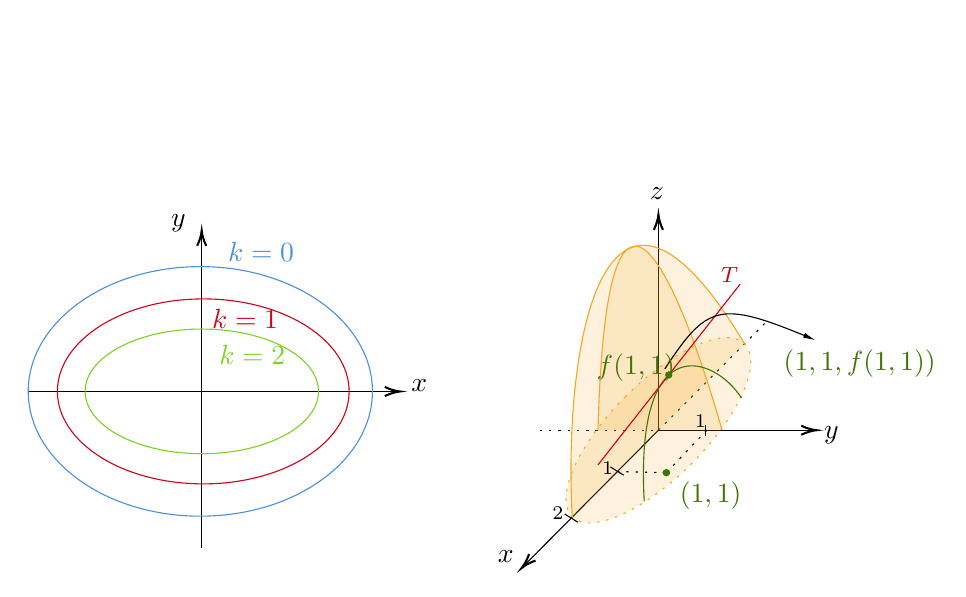
\begin{tikzpicture}[x=0.5pt,y=0.5pt,yscale=-1,xscale=1]
                    %Straight Lines [id:da6780406550785627] 
                    \draw    (509.65,187.67) -- (509.65,33.89) ;
                    \draw [shift={(509.65,31.89)}, rotate = 90] [color={rgb, 255:red, 0; green, 0; blue, 0 }  ][line width=0.75]    (10.93,-3.29) .. controls (6.95,-1.4) and (3.31,-0.3) .. (0,0) .. controls (3.31,0.3) and (6.95,1.4) .. (10.93,3.29)   ;
                    %Straight Lines [id:da38857849447173476] 
                    \draw    (509.65,187.67) -- (621.82,187.67) ;
                    \draw [shift={(623.82,187.67)}, rotate = 180] [color={rgb, 255:red, 0; green, 0; blue, 0 }  ][line width=0.75]    (10.93,-3.29) .. controls (6.95,-1.4) and (3.31,-0.3) .. (0,0) .. controls (3.31,0.3) and (6.95,1.4) .. (10.93,3.29)   ;
                    %Straight Lines [id:da34960806629184693] 
                    \draw    (509.65,187.67) -- (412.22,285.85) ;
                    \draw [shift={(410.81,287.27)}, rotate = 314.78] [color={rgb, 255:red, 0; green, 0; blue, 0 }  ][line width=0.75]    (10.93,-3.29) .. controls (6.95,-1.4) and (3.31,-0.3) .. (0,0) .. controls (3.31,0.3) and (6.95,1.4) .. (10.93,3.29)   ;
                    %Straight Lines [id:da1115594625878652] 
                    \draw  [dash pattern={on 0.84pt off 2.51pt}]  (509.65,187.67) -- (589.5,107.49) ;
                    %Straight Lines [id:da1437148228723495] 
                    \draw  [dash pattern={on 0.84pt off 2.51pt}]  (423.97,187.67) -- (509.65,187.67) ;
                    %Flowchart: Connector [id:dp5111535006556838] 
                    \draw  [color={rgb, 255:red, 245; green, 166; blue, 35 }  ,draw opacity=1 ][fill={rgb, 255:red, 245; green, 166; blue, 35 }  ,fill opacity=0.15 ][dash pattern={on 0.84pt off 2.51pt}] (485.55,163.63) .. controls (519.94,129.15) and (558.61,111.95) .. (571.92,125.23) .. controls (585.23,138.5) and (568.14,177.21) .. (533.75,211.7) .. controls (499.36,246.19) and (460.69,263.38) .. (447.38,250.11) .. controls (434.07,236.83) and (451.16,198.12) .. (485.55,163.63) -- cycle ;
                    %Curve Lines [id:da4882972292661457] 
                    \draw [color={rgb, 255:red, 245; green, 166; blue, 35 }  ,draw opacity=1 ][fill={rgb, 255:red, 245; green, 166; blue, 35 }  ,fill opacity=0.15 ]   (447.38,250.11) .. controls (440.51,122.65) and (471.52,-42.74) .. (571.92,125.23) ;
                    %Curve Lines [id:da389646540747271] 
                    \draw [color={rgb, 255:red, 245; green, 166; blue, 35 }  ,draw opacity=1 ][fill={rgb, 255:red, 245; green, 166; blue, 35 }  ,fill opacity=0.15 ]   (466,187.43) .. controls (473.95,-102.86) and (550.77,170.89) .. (555.59,187.43) ;
                    %Straight Lines [id:da4028057377695208] 
                    \draw    (441.88,248.19) -- (451.53,254.16) ;
                    %Straight Lines [id:da3007863113327215] 
                    \draw    (474.96,214.19) -- (484.61,220.17) ;
                    %Straight Lines [id:da12798592457241997] 
                    \draw    (543.42,183.87) -- (543.42,192.14) ;
                    %Straight Lines [id:da898081741331547] 
                    \draw  [dash pattern={on 0.84pt off 2.51pt}]  (544.57,187.67) -- (515.39,218.33) ;
                    %Straight Lines [id:da02616518172359583] 
                    \draw  [dash pattern={on 0.84pt off 2.51pt}]  (479.79,217.53) -- (515.39,218.33) ;
                    %Shape: Ellipse [id:dp4201828680741282] 
                    \draw  [draw opacity=0][fill={rgb, 255:red, 65; green, 117; blue, 5 }  ,fill opacity=1 ] (512.56,218.33) .. controls (512.56,216.86) and (513.83,215.67) .. (515.39,215.67) .. controls (516.96,215.67) and (518.23,216.86) .. (518.23,218.33) .. controls (518.23,219.8) and (516.96,220.98) .. (515.39,220.98) .. controls (513.83,220.98) and (512.56,219.8) .. (512.56,218.33) -- cycle ;
                    %Curve Lines [id:da41685873274751206] 
                    \draw [color={rgb, 255:red, 65; green, 117; blue, 5 }  ,draw opacity=1 ]   (499.38,238.82) .. controls (492.5,111.37) and (551.14,134.88) .. (569.67,164.4) ;
                    %Straight Lines [id:da10089497266497283] 
                    \draw [color={rgb, 255:red, 208; green, 2; blue, 27 }  ,draw opacity=1 ]   (568.7,82.13) -- (517.12,147.69) -- (465.93,212.75) ;
                    %Shape: Ellipse [id:dp6247799862140714] 
                    \draw  [draw opacity=0][fill={rgb, 255:red, 65; green, 117; blue, 5 }  ,fill opacity=1 ] (514.47,147.69) .. controls (514.47,146.23) and (515.66,145.05) .. (517.12,145.05) .. controls (518.57,145.05) and (519.76,146.23) .. (519.76,147.69) .. controls (519.76,149.15) and (518.57,150.33) .. (517.12,150.33) .. controls (515.66,150.33) and (514.47,149.15) .. (514.47,147.69) -- cycle ;
                    %Curve Lines [id:da66732394411051] 
                    \draw [color={rgb, 255:red, 0; green, 0; blue, 0 }  ,draw opacity=1 ]   (514.29,143.35) .. controls (544.92,96.72) and (553.71,93.76) .. (618.07,120.43) ;
                    \draw [shift={(619.04,120.84)}, rotate = 202.56] [color={rgb, 255:red, 0; green, 0; blue, 0 }  ,draw opacity=1 ][line width=0.75]    (4.37,-1.32) .. controls (2.78,-0.56) and (1.32,-0.12) .. (0,0) .. controls (1.32,0.12) and (2.78,0.56) .. (4.37,1.32)   ;
                    %Straight Lines [id:da7981422257753735] 
                    \draw    (179.59,272.5) -- (179.59,45.45) ;
                    \draw [shift={(179.59,43.45)}, rotate = 90] [color={rgb, 255:red, 0; green, 0; blue, 0 }  ][line width=0.75]    (10.93,-3.29) .. controls (6.95,-1.4) and (3.31,-0.3) .. (0,0) .. controls (3.31,0.3) and (6.95,1.4) .. (10.93,3.29)   ;
                    %Straight Lines [id:da1510535259545942] 
                    \draw    (54.22,159.67) -- (320.87,159.67) ;
                    \draw [shift={(322.87,159.67)}, rotate = 180] [color={rgb, 255:red, 0; green, 0; blue, 0 }  ][line width=0.75]    (10.93,-3.29) .. controls (6.95,-1.4) and (3.31,-0.3) .. (0,0) .. controls (3.31,0.3) and (6.95,1.4) .. (10.93,3.29)   ;
                    %Shape: Ellipse [id:dp38778929607653] 
                    \draw  [color={rgb, 255:red, 126; green, 211; blue, 33 }  ,draw opacity=1 ] (95.33,159.6) .. controls (95.33,134.72) and (133.08,114.54) .. (179.66,114.54) .. controls (226.23,114.54) and (263.98,134.72) .. (263.98,159.6) .. controls (263.98,184.48) and (226.23,204.65) .. (179.66,204.65) .. controls (133.08,204.65) and (95.33,184.48) .. (95.33,159.6) -- cycle ;
                    %Shape: Ellipse [id:dp7875438618467064] 
                    \draw  [color={rgb, 255:red, 208; green, 2; blue, 27 }  ,draw opacity=1 ] (75.3,159.6) .. controls (75.3,122.69) and (122.5,92.76) .. (180.71,92.76) .. controls (238.92,92.76) and (286.12,122.69) .. (286.12,159.6) .. controls (286.12,196.51) and (238.92,226.44) .. (180.71,226.44) .. controls (122.5,226.44) and (75.3,196.51) .. (75.3,159.6) -- cycle ;
                    %Shape: Ellipse [id:dp9439316502559274] 
                    \draw  [color={rgb, 255:red, 74; green, 144; blue, 226 }  ,draw opacity=1 ] (54.22,159.6) .. controls (54.22,109.8) and (109.91,69.42) .. (178.6,69.42) .. controls (247.29,69.42) and (302.98,109.8) .. (302.98,159.6) .. controls (302.98,209.4) and (247.29,249.78) .. (178.6,249.78) .. controls (109.91,249.78) and (54.22,209.4) .. (54.22,159.6) -- cycle ;

                    % Text Node
                    \draw (391.8,272.52) node [anchor=north west][inner sep=0.75pt]  [font=\normalsize]  {$x$};
                    % Text Node
                    \draw (501.51,10.61) node [anchor=north west][inner sep=0.75pt]  [font=\normalsize]  {$z$};
                    % Text Node
                    \draw (627.6,182.98) node [anchor=north west][inner sep=0.75pt]  [font=\normalsize]  {$y$};
                    % Text Node
                    \draw (431.2,241.62) node [anchor=north west][inner sep=0.75pt]  [font=\scriptsize]  {$2$};
                    % Text Node
                    \draw (467.03,209) node [anchor=north west][inner sep=0.75pt]  [font=\scriptsize]  {$1$};
                    % Text Node
                    \draw (534.11,175) node [anchor=north west][inner sep=0.75pt]  [font=\scriptsize]  {$1$};
                    % Text Node
                    \draw (523.26,223.03) node [anchor=north west][inner sep=0.75pt]  [font=\normalsize]  {$\textcolor[rgb]{0.25,0.46,0.02}{(}\textcolor[rgb]{0.25,0.46,0.02}{1,1}\textcolor[rgb]{0.25,0.46,0.02}{)}$};
                    % Text Node
                    \draw (463.19,130.45) node [anchor=north west][inner sep=0.75pt]  [font=\normalsize]  {$\textcolor[rgb]{0.25,0.46,0.02}{f}\textcolor[rgb]{0.25,0.46,0.02}{(}\textcolor[rgb]{0.25,0.46,0.02}{1,1}\textcolor[rgb]{0.25,0.46,0.02}{)}$};
                    % Text Node
                    \draw (553.15,67.78) node [anchor=north west][inner sep=0.75pt]  [font=\footnotesize,color={rgb, 255:red, 208; green, 2; blue, 27 }  ,opacity=1 ]  {$T$};
                    % Text Node
                    \draw (598.33,127.66) node [anchor=north west][inner sep=0.75pt]  [font=\normalsize]  {$\textcolor[rgb]{0.25,0.46,0.02}{(}\textcolor[rgb]{0.25,0.46,0.02}{1,1,f}\textcolor[rgb]{0.25,0.46,0.02}{(}\textcolor[rgb]{0.25,0.46,0.02}{1,1}\textcolor[rgb]{0.25,0.46,0.02}{)}\textcolor[rgb]{0.25,0.46,0.02}{)}$};
                    % Text Node
                    \draw (329.14,149.04) node [anchor=north west][inner sep=0.75pt]  [font=\normalsize]  {$x$};
                    % Text Node
                    \draw (155.67,30.01) node [anchor=north west][inner sep=0.75pt]  [font=\normalsize]  {$y$};
                    % Text Node
                    \draw (190.39,124.12) node [anchor=north west][inner sep=0.75pt]  [font=\normalsize]  {$\textcolor[rgb]{0.49,0.83,0.13}{k=2}$};
                    % Text Node
                    \draw (185.16,98.1) node [anchor=north west][inner sep=0.75pt]  [font=\normalsize]  {$\textcolor[rgb]{0.82,0.01,0.11}{k=1}$};
                    % Text Node
                    \draw (196.74,49.75) node [anchor=north west][inner sep=0.75pt]  [font=\normalsize]  {$\textcolor[rgb]{0.29,0.56,0.89}{k=0}$};
                \end{tikzpicture}
        \caption{Interpretação geométrica da derivada de \(f(x,y) = 4 - x^2 - y^2\)}
        \label{fig:derivada1}
    \end{figure}

    Para \(\partial_xf(1,1)\), fixamos \(y=1\) e assim o gráfico de \(g(x) = f(x,1) = 2 - x^2\) é uma parábola que é a interseção do plano \(y=1\) com o gráfico de \(f\). Como já vimos, o coeficiente angular da reta tangente \(T\) à parábola no ponto \((1,1,1)\) é \[g'(1) = \partial_xf(1,1) = -2 = \tan(\theta).\] 
    
    A interpretação geométrica para \(\partial_yf(1,1)\) fica de exercício.    
\end{example}

\begin{example}
    Estude as derivadas parciais de \(f(x,y) = \begin{cases}
        \frac{x^3 - y^2}{x^2 + y^2},\; (x,y)\neq(0,0) \\
        0,\; (x,y)=(0,0).
    \end{cases}\) 

    Vamos começar estudando \(\frac{\partial f}{\partial x}\)
        \begin{itemize}
            \item Se \((x,y) \neq (0,0)\), temos \[\partial_xf(x,y) = \frac{3x^2(x^2+y^2) - (x^3-y^2)2x}{(x^2+y^2)^2}.\]
            \item Se \((x,y)=(0,0)\), \[\partial_xf(0,0) = \lim_{x\to 0} \frac{f(x,0)-f(0,0)}{x-0} = \lim_{x\to 0} \frac{x}{x} = \lim_{t\to 0} 1 = 1.\]
        \end{itemize}
    Portanto \[\frac{\partial f}{\partial x}(x,y) = \begin{cases}
        \frac{x^4 + 3x^2y^2 + 2xy^2}{(x^2+y^2)^2},\; (x,y)\neq(0,0) \\
        1,\; (x,y)=(0,0)
    \end{cases}\]

    Agora, para \(\frac{\partial f}{\partial y}\),
    \begin{itemize}
        \item Se \((x,y)\neq(0,0)\), \[\partial_yf(x,y) = \frac{-2y(x^2+y^2)-(x^3-y^2)2y}{(x^2+y^2)^2} = \frac{-2x^2y - 2x^3y}{(x^2+y^2)^2},\]
        \item se \((x,y)=(0,0)\), \[\partial_yf(0,0) = \lim_{y\to 0} \frac{f(0,y)-f(0,0)}{y} = \lim_{y\to 0} -\frac{1}{y} = -\infty.\]
    \end{itemize}
    Portanto \(\partial_y f(x,y)\) está definida apenas para \((x,y)\neq(0,0)\).
\end{example}

\begin{proposition}
    Seja \(f:\R^2\to\R\) tal que \(\frac{\partial f}{\partial x}(x,y) = 0\), para todo \((x,y)\in\R^2\). Então \(f\) não depende de \(x\), ou seja, existe \(\phi:\R\to\R\) tal que \(f(x,y) = \phi(y),\) para todo \((x,y)\in\R 2\).
\end{proposition}

\begin{proof}
    Fixado \(y_0\in\R\), considere a função \[h(x) = f(x,y_0),\; x\in\R.\] Então \[h'(x) = \partial_xf(x,y_0) = 0\,; \forall x\in\R,\] ou seja, \(h\) é contínua (dado que é diferenciável) e \(h'(x) = 0\), para todo \(x\in\R\). Segue então que \(h\) é constante em \(\R\). Portanto \[h(x) = h(0),\;\forall x\in\R,\] daí \[f(x,y_0) = f(0,y_0),\;\forall x\in\R.\] Como \(y_0\in\R\) é arbitrário, segue que \[f(x,y) = f(0,y),\; \forall(x,y)\in\R^2.\] Tomando \(\phi(y) = f(0,y)\) temos que \[f(x,y) = \phi(y),\; \forall(x,y)\in\R^2.\]
\end{proof}

\section{Derivadas de funções definidas implicitamente}

Dada a equação \[z = \sqrt{1 - x^2 - y^2},\; x^2 + y^2 < 1\] dizemos que \(z\) é uma \textbf{função explícita} de \((x,y)\), pois podemos escrever \(z = f(x,y)\), com \(f(x,y) = \sqrt{1 - x^2 - y^2}\) e \(D_f = \{(x,y)\in\R^2 : x^2 + y^2 < 1\}\).

No entanto, a equação
\begin{equation}\label{eq.esfera}
    x^2 + y^2 + z^2 - 1 = 0,\; z>0
\end{equation}
define a mesma função \(f\), uma vez que isolando \(z\) em função de \(x\) e \(y\) temos \[z^2 = 1 - x^2 - y^2 \Rightarrow z = \sqrt{1-x^2-y^2},\; x^2 + y^2 < 1.\] Neste caso dizemos que \(z = f(x,y)\) está definida \textbf{implicitamente} pela equação \eqref{eq.esfera}.

\begin{remark}
    Note que considerando \(g(x,y,z) = x^2 + y^2 + z^2 -1\) e \(f(x,y) = \sqrt{1-x^2-y^2}\), com \(x^2 + y^2 < 1\), e substituindo \(z = f(x,y)\), com \((x,y)\in D_f\), em \(g(x,y,z)\) obtemos \[g(x,y,f(x,y)) = x^2 + y^2 + (\sqrt{1-x^2-y^2})^2 - 1 = x^2 + y^2 + 1 - x^2 - y^2 - 1 = 0.\] Ou seja, \((x,y,f(x,y))\) satisfaz a equação \[g(x,y,z) = 0.\]

    Esta é uma característica de toda função definida implicitamente por uma equação nas variáveis \(x, y\) e \(z\). Logo, em geral, temos a seguinte caracterização:
\end{remark}

\begin{definition}
    Uma função \(z = f(x,y)\) é \textbf{definida implicitamente} pela equação \(g(x,y,z) = 0\) se, para todo \((x,y)\in D_f\), \(g(x,y,f(x,y)) = 0.\)
\end{definition}

\begin{remark}
    É importante notar que:
        \begin{enumerate}
            \item Nem toda função \(z = f(x,y)\) definida implicitamente por uma equação \(g(x,y,f(x,y)) = 0\) pode ser colocada de maneira explícita. Portanto a caracterização acima é importante.
            \item A caracterização acima implica que o gráfico da função implícita coincide com \textit{uma parte do} (ou todo o) gráfico da equação.
        \end{enumerate}
\end{remark}

\begin{exercise}
    Verifique que as funções
        \begin{align*}
            z & = \sqrt{1-x^2-y^2},\; x^2 + y^2 \leq 1 \\
            z & = - \sqrt{1-x^2-y^2},\; x^2 + y^2 \leq 1
        \end{align*}
também são definidas pela equação \[x^2 + y^2 + z^2 - 1 = 0.\]
\end{exercise}

\begin{example}
    Seja \(z = f(x,y)\) dada implicitamente por \[x^2 + y^2 + z^2 = 1.\] Calcule \(\frac{\partial z}{\partial x}\) e \(\frac{\partial z}{\partial y}\).

    Para calcular \(\frac{\partial z}{\partial x}\) notamos que isolando \(z\) na equação dada obtemos \[z = \sqrt{1 - x^2 - y^2},\; x^2 + y^2 < 1,\] logo \[\frac{\partial z}{\partial x} = \frac{\partial}{\partial x} \sqrt{1-x^2-y^2} = \frac{1}{2}(1-x^2-y^2)^\frac{1}{2}\cdot(2x) = -\frac{x}{\sqrt{1-x^2-y^2}},\] ou seja, \[\frac{\partial z}{\partial x} = - \frac{x}{\sqrt{1-x^2-y^2}},\; x^2 + y^2 < 1.\]

    Podemos também calcular \(\frac{\partial z}{\partial x}\) trabalhando diretamente com a equação dada. Neste caso
        \begin{align*}
            \frac{\partial}{\partial x} (x^2 + y^2 + z^2) = \frac{\partial}{\partial x}(1)
            \Rightarrow & \frac{\partial}{\partial x} (x^2 + y^2) + \frac{\partial}{\partial x} z^2 = 0 \\
            \Rightarrow & 2x + \frac{d}{dz}z^2\cdot\frac{\partial z}{\partial x} = 0 \\
            \Rightarrow & 2x + 2z\cdot\frac{\partial z}{\partial x} = 0 \\
            \Rightarrow & \frac{\partial z}{\partial x} = -\frac{x}{z} = \frac{-x}{\sqrt{1-x^2-y^2}},; x^2 + y^2 < 1.
        \end{align*}
\end{example}

\section{Derivadas parciais de ordem superior}

\section{Funções diferenciáveis}

\section{Diferencial}

\section{Vetor gradiente}

\section{Regra da cadeia}



\section{Teorema da função implícita}

\section{Gradiente e derivada direcional}

\section{Fórmula de Taylor}

\section{Máximos e mínimos}

\section{Máximos e mínimos em conjuntos compactos}

\section{Método dos multiplicadores de Lagrange: Máximos e mínimos condicionados}

